\graphicspath{{images/act_1.6/}}
\subsection{Cartesian space PD control + gravity compensation}
The objective of this activity is to control movement of the ur5 robot end-effector so that it follows the Cartesian step reference trajectory of activity \ref{subsec:generate_step_reference}. The simulation starts with initial joint configuration $\mathbf{q_0}=\begin{bmatrix} 0.0 & -1.0 & 1.0 & 0.5 & 0.0 & 0.5 \end{bmatrix}$ rad and end-effector $\mathbf{p_0}=\begin{bmatrix}  0.577 &   0.192 &   0.364 \end{bmatrix}$~m. Likewise, the Cartesian step reference trajectory starts at $\mathbf{p_0}$. Motion control is made up of two approaches: proportional-derivative with gravity compensation at the Cartesian level and projection of the null space. In this sense, the PD$+$g control method contributes with the reduction of trajectory tracking error and the projection of null space maintains the articular position close to~$\mathbf{q_0}$. Finally, control law can be computed as 
\begin{equation}
	\boldsymbol{\tau}
	= \mathbf{J^T} (\mathbf{K_p e} + \mathbf{K_d \dot{e}}+ \mathbf{J^{T\#} g}) + \mathbf{N} \left(\mathbf{K_q(q_0-q) - D_q \dot{q}} \right),
	\label{eq:cartesian_PD_control_g_null_space}
\end{equation}
\begin{equation*}
	\mathbf{N}=(\mathbf{I_{6 \times 6}} - \mathbf{J^{\#} J} ),
\end{equation*}
\noindent where $\mathbf{J}$ is jacobian matrix, $\mathbf{e}=\mathbf{p_{des} - p}$ is end-effector position error, $\mathbf{K_p, K_d}$ are the proportional and derivative gains respectively, $\mathbf{J^{\#}}$ is jacobian damped pseudo-inverse, $\mathbf{g}$ is gravity compensation term, $\mathbf{N}$ is the null space projection of $\mathbf{J^{\#}}$, and $\mathbf{K_q, D_q}$ are the proportional and derivative gains for null space projection. \vspace{.5cm}

The Algorithm \ref{lst:cartesian_PD_control_g_postural_task} control the movements of ur5 robot end-effector to track the Cartesian step reference trajectory of activity~\ref{subsec:generate_step_reference}. In this file, the PD control method is configured with ${K_{p}}=1000$ $\mathrm{\frac{N}{m}}$ and $K_{d}= 300$ $\mathrm{\frac{N.s}{m}}$ and the null space projection is configured with ${K_{q}}=50$ $\mathrm{\frac{N.m}{rad}}$ and $K_{d}= 10$ $\mathrm{\frac{N.m.s}{rad}}$. On one hand, Figure \ref{fig:act_1.6_ee_position} shows that trajectory tracking performance at the Cartesian space is good with mean norm error at each axis ($||e_x||, ||e_y||, ||e_z||$) of $0.0002$, $0.0001$, $0.025$ cm respectively. The gravity term in control law \eqref{eq:cartesian_PD_control_g_null_space} reduces the position error in $z$-axis from $0.08$ cm (obtained in activity \ref{subsec:cartesian_PD_control_postural_task}) to $0.025$ cm. On the other hand, Figure \ref{fig:act_1.6_joint_position} shows that angular trajectory of each joint with a PD at Cartesian space is different from angular trajectory obtained with a PD at joint space in activity \ref{subsec:inverse_kinematics_approach}. This is because the control law focuses on reducing the Cartesian position error of the end effector rather than position error of each joint. Finally, null space projection allows the smooth variation of the position of each joint, so the system remained stable for the entire simulation unlike activity \ref{subsec:cartesian_space_PD_control}. \vspace{.5cm}

\begin{lstlisting}[language=Python,caption=Move the ur5 robot end-effector using PD control method with gravity compensation and null space projection to follows the Cartesian step reference trajectory of activity \ref{subsec:generate_step_reference}., label={lst:cartesian_PD_control_g_postural_task}]

# =========================
#   Configuration of node
# =========================
# create a node: 
rospy.init_node("cartesian_space_PD_control_postural_task_gravity_compensation")
# public in topic /joint_states	to send joint data	
pub = rospy.Publisher('joint_states', JointState, queue_size=1000)
# loop rate (in Hz)
rate 	= rospy.Rate(1000)		# 1000 [Hz]
dt 		= 1e-3					# 1  [ms]
# object(message) type JointState
jstate = JointState()

# ==========================================
#   Set initial joint configuration of UR5
# ==========================================
# initial configuration: position, velocity and acceleration 
q0 =   np.array([ 0.0, -1.0, 1.0, 0.5, 0.0, 0.5])
dq0 =  np.array([0.0, 0.0, 0.0, 0.0, 0.0, 0.0]) 
ddq0 = np.array([0.0, 0.0, 0.0, 0.0, 0.0, 0.0]) 

# desired trajectory: position, velocity and acceleration
q_des =   np.array([ 0.0, -1.0, 1.0, 0.5, 0.0, 0.5])
dq_des =  np.array([0.0, 0.0, 0.0, 0.0, 0.0, 0.0]) 
ddq_des = np.array([0.0, 0.0, 0.0, 0.0, 0.0, 0.0]) 

# measured trajectory: position, velocity and acceleration
q_med =   np.array([ 0.0, -1.0, 1.0, 0.5, 0.0, 0.5])
dq_med =  np.array([0.0, 0.0, 0.0, 0.0, 0.0, 0.0]) 
ddq_med = np.array([0.0, 0.0, 0.0, 0.0, 0.0, 0.0]) 

# ===========================
#   UR5 robot configuration
# ===========================
# joints name of UR5 robot
jnames = ['shoulder_pan_joint', 'shoulder_lift_joint', 'elbow_joint','wrist_1_joint', 'wrist_2_joint', 'wrist_3_joint']
# path of labs_ur5.urdf
urdf_path = os.path.join(pwd, "../../ur5_description/urdf/labs_ur5.urdf")
# the class robot load labs_ur5.urdf
ur5_robot = Robot(q0, dq0, dt, urdf_path)
# number of degress of freedom
ndof = ur5_robot.ndof

# create inertia matrix 
M = np.zeros([ndof,ndof])
# create nonlinear effects vector
b = np.zeros(ndof)
# create gravity vector
g = np.zeros(ndof)

# ==============================================
#   set initial cartesian configuration of UR5
# ==============================================
# initial cartesian configuration: position, velocity and acceleration
p0 = ur5_robot.get_ee_position()
dp0 = np.array([0.0, 0.0, 0.0])
ddp0 = np.array([0.0, 0.0, 0.0])

# desired cartesian trajectory: position, velocity and acceleration
p_des = copy(p0)
dp_des = np.array([0.0, 0.0, 0.0])
ddp_des = np.array([0.0, 0.0, 0.0])

# measured cartesian trajectory: position, velocity and acceleration
p_med = copy(p0)
dp_med = np.array([0.0, 0.0, 0.0])
ddp_med = np.array([0.0, 0.0, 0.0])

# ===============================
#   PD controller configuration
# ===============================
# proportional gain
kp = np.array([1000, 1000, 1000])   # N/m
# derivative gain   
kd = np.array([300, 300, 300])      # N.s/m
# control vector
tau_PD = np.zeros(ndof)    

# postural task: gains
Kq = 50*np.eye(ndof)
Dq = 10*np.eye(ndof)
# postural task: control term
tau_0 = np.zeros(ndof)

#===============
#   Simulation
#===============
t = 0.0             # [sec] 
sim_duration = 5.0  # [sec]
step_start = 2.0    # [sec]

while not rospy.is_shutdown():
    # desired cartesian trajectory
    p_des[2], dp_des[2], ddp_des[2] = step_reference_generator(p0[2], 0.1, step_start, t)

    # jacobian: position xyz [3x6]
    J = ur5_robot.jacobian(q_des)[0:3, 0:6]  
    # jacobian: damped pseudo-inverse [6x3]
    J_inv = ur5_robot.jacobian_damped_pinv(J)   

    # error: position and velocity
    e 	=  p_des - p_med
    de 	=  dp_des - dp_med    

    # dynamics: gravity term
    g = ur5_robot.get_g()

    # postural task: control term
    tau_0 = Kq.dot(q0-q_med) - Dq.dot(dq_med)
    N = np.eye(ndof) - J_inv.dot(J)
    
    # PD + gravity compensation (cartesian space)
    tau_PD = J.T.dot( np.multiply(kp, e) + np.multiply(kd, de) + J_inv.T.dot(g))
    # control signal: PD + g + null space projection
    tau = tau_PD + N.dot(tau_0)
    
    # send control signal
    ur5_robot.send_control_command(tau)
    # update states
    q_med, dq_med, ddq_med = ur5_robot.read_joint_position_velocity_acceleration()
    p_med, dp_med, ddp_med = ur5_robot.read_cartesian_position_velocity_acceleration()

    # publish message
    jstate.header.stamp = rospy.Time.now()
    jstate.name 		= jnames			# Joints position name
    jstate.position 	= q_med
    jstate.velocity 	= dq_med
    pub.publish(jstate)

    # update time
    t = t + dt

    # stop simulation
    if t>=sim_duration:
        print("stopping rviz ...")
        break
    rate.sleep()
\end{lstlisting}




\vspace*{0cm}
\begin{figure}[H]
	\centering
	\subfloat[]{
	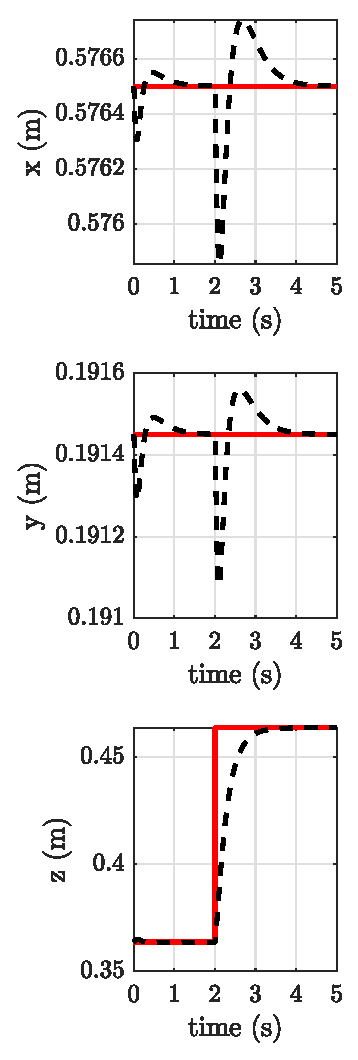
\includegraphics{ee_position.eps}
	}
	%\hfill
	\subfloat[]{
	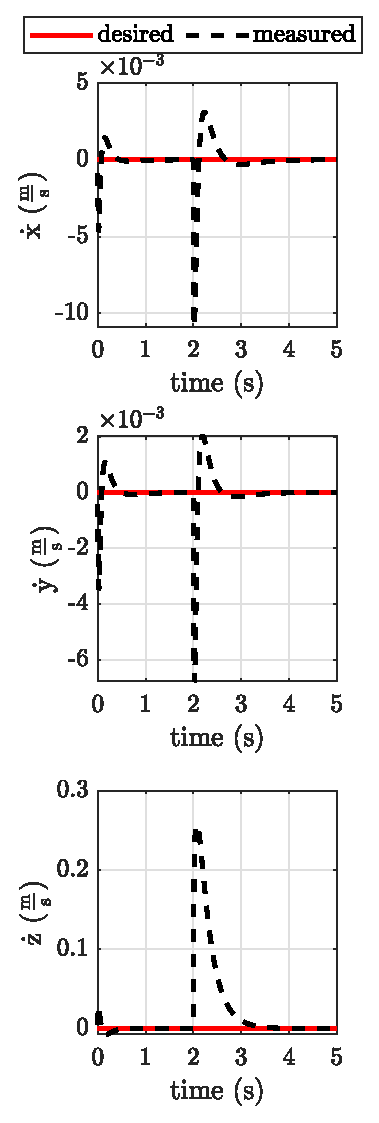
\includegraphics{ee_velocity.eps}
	}	
	%\hfill
	\subfloat[]{
	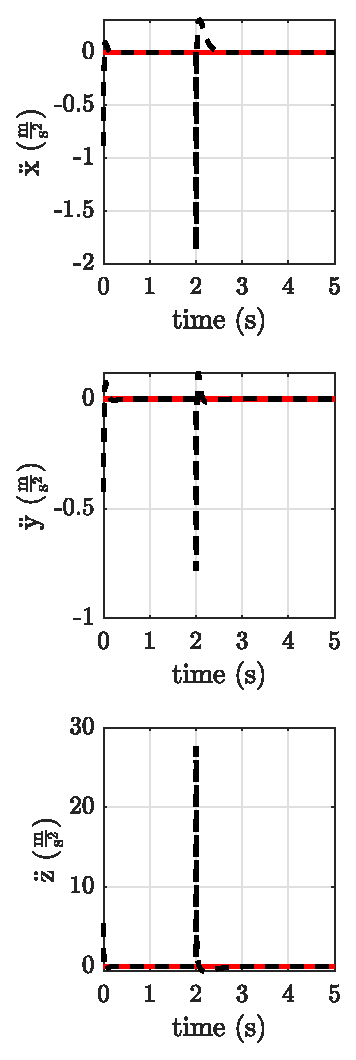
\includegraphics{ee_acceleration.eps}
	}		
	\caption{Trajectory tracking performances of the control method \eqref{eq:cartesian_PD_control_g_null_space} with  ${K_{p}}=1000$ $\mathrm{\frac{N}{m}}$, $K_{d}= 300$ $\mathrm{\frac{N.s}{m}}$, ${K_{q}}=50$ $\mathrm{\frac{N.m}{rad}}$, $K_{d}= 10$ $\mathrm{\frac{N.m.s}{rad}}$: (a) position, (b) velocity and (c) acceleration.}
	\label{fig:act_1.6_ee_position}
\end{figure}

\begin{figure}
    \centering
    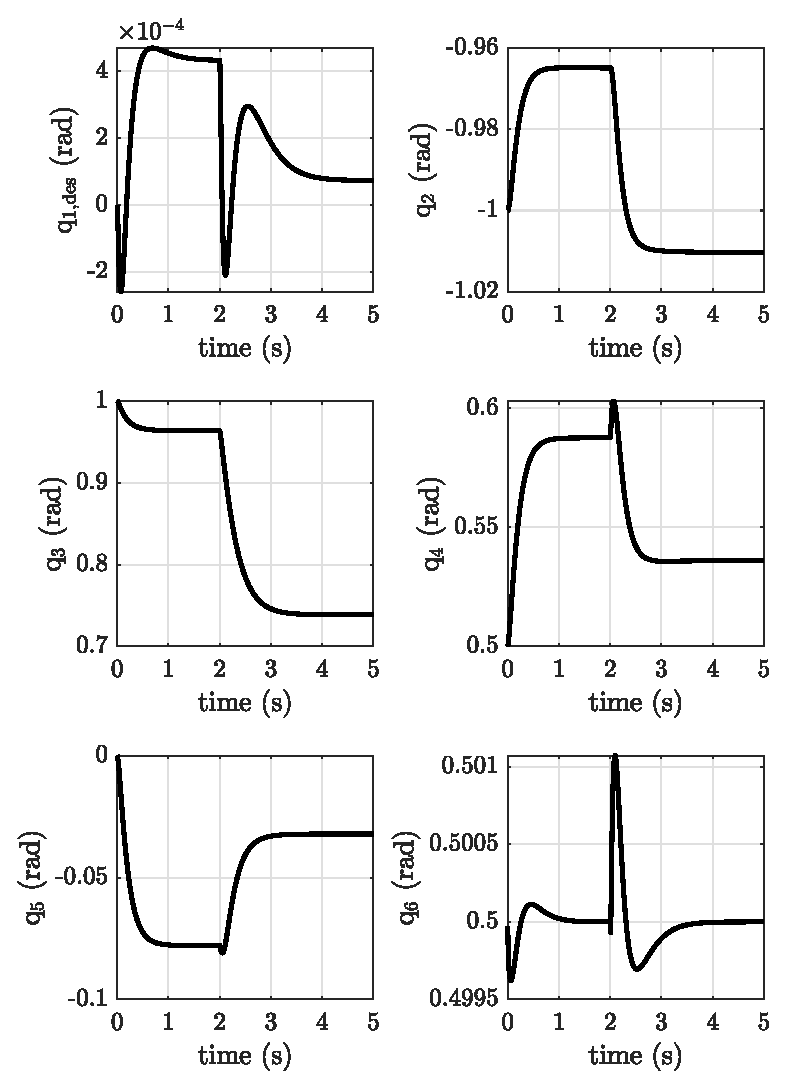
\includegraphics{joint_position.eps}	
    \caption{Angular position of each joint of UR5 robot with Algorithm \ref{lst:cartesian_PD_control_g_postural_task}.}
    \label{fig:act_1.6_joint_position}
\end{figure}